%%%%%%%%%%%%%%%%%%%%%%%%%%%%%%%%%%%%%%%%%%%%%%%%%%%%%%%%%%%%%%%%%%%%%%%%%%%%%%%%%%%%%%%%%%%%%
%CHAPTER 1%%%%%%%%%%%%%%%%%%%%%%%%%%%%%%%%%%%%%%%%%%%%%%%%%%%%%%%%%%%%%%%%%%%%%%%%%%%%%%%%%%%
%%%%%%%%%%%%%%%%%%%%%%%%%%%%%%%%%%%%%%%%%%%%%%%%%%%%%%%%%%%%%%%%%%%%%%%%%%%%%%%%%%%%%%%%%%%%%
\chapter{Linear Algebra in Finite dimensions}

In this chapter we will discuss linear algebra in vector spaces that have finite dimension.  These are the vector spaces that are probably most familiar to you, such as the space \textbf{R}$^{n}$ studied in introductory linear algebra courses.  Our emphasis will be on understanding vectors as objects independent of the particular choice of basis that is used to represent them.  We will then look at linear transformations of vectors and see how they're represented by matrices.  We will see that the matrix representation of a linear transformation is not unique; it depends on the basis that you're using.  To tie the ideas together and to show why these things are of interest to a physicist we will use all of our mathematical machinery on a certain physical system that appears complicated: the coupled oscillator.  By the end of this chapter we will be able to solve the equations of motion for this system in an elegant and very easy way.

The beginnings and ends of sections discussing this physical system will be marked by a $\clubsuit$ to set them apart from the rest of the text.

\section{Introduction - The Big Picture}
In this section I'm going to explain the main message of this chapter, and actually this entire document, by dissecting an extremely simple idea in great detail.
In linear algebra class the archetypical vector space is the set of lists of $n$ numbers, $\textbf{R}^n$.
It's easy to see that things are indeed vectors: you can add them together and multiply them by scalars \footnote{For example, $(1,4,3)+(0,1,5)=(1,5,8)$}  $\textbf{R}^n$, but rather we use elements in $\textbf{R}^n$, namely lists of numbers, to represent the things we \emph{are} interested in.
For example, we can use lists of two numbers to represent displacement in a two dimensional plane.
In figure \ref{Fig} we draw a plane with a coordinate system and two arrows \textbf{v} and \textbf{w}, each of unit length.
If we let $\ket{x}$ represent a unit arrow along the $x$ axis and $\ket{y}$ represent a unit arrow along the $y$ axis, then our two arrows are represented as,
\begin{equation}
\ket{v} \sim \frac{1}{\sqrt{2}} \left[ \begin{array}{c} 1 \\ 1 \end{array} \right] \
\qquad \ket{w} \sim \frac{1}{\sqrt{2}} \left[ \begin{array}{c} 1 \\ -1 \end{array} \right]
\end{equation}
If you add the lists together you get $(\sqrt{2},0)$ which is of course the correct representation for the geometric sum of the two arrows.

We could choose another set of coordinate axes as in Figure \ref{Fig}.
Call the arrows with unit length along these axes $\ket{p}$ and $\ket{q}$.
Then our arrows are represented as
\begin{displaymath}
\ket{v}\sim \left[\begin{array}{c} 1 \\ 0 \end{array} \right] \qquad \
\ket{w}\sim \left[\begin{array}{c} 0 \\ -1 \end{array} \right]
\end{displaymath}
The arrow $\ket{v}$ didn't change but the vector in $\textbf{R}^2$ did.
This highlights the most essential philosophical point to be made in this document: 

\section{The Coupled Oscillator}
Consider the system shown in \ref{Fig:CoupledMasses} consisting of two boxes of equal mass $m$ connected by three springs of equal spring constant $k$.  A natural question is, given initial positions and velocities of the boxes at time $t_{0}$ what are their positions and velocities at another time $t$?  To answer this question we have to solve Newton's equation for each box.  This is not so easy.  The equations of motion (Newton's equations) for the boxes are
\begin{equation} \label{eq:Newton}
\ddot{x}_{1} = \omega_{0}^{2} (-2x_{1} + x_{2}) \qquad
\ddot{x}_{2} = \omega_{0}^{2} (-2x_{2} + x_{1})
\end{equation}
where $\omega^{2}_{0} = \frac{k}{m}$.  This is a set of two second order differential equations which are \textit{coupled}, meaning that each equation has dependance on both $x_1$ and $x_2$.  To the untrained eye it looks very difficult to solve.  You are urged to try to solve for $x_{1}(t)$ and $x_{2}(t)$ so that you will appreciate the power of what is to come.

\begin{figure}
\begin{centering}
\includegraphics[width=12cm]{boxes.pdf}
\par\end{centering}
\caption{Coupled mass system. Each spring has spring constant $k$ and each box has mass $m$. The walls are fixed in place.}
\label{Fig:CoupledMasses}
\end{figure}

\begin{flushleft}\textbf{Exercises}\end{flushleft} %Exercises
\begin{itemize}\item[1)] Verify that (\ref{eq:Newton}) correctly describes the motion of the two coupled masses.\item[2)] Try to solve for $x_{1}(t)$ and $x_{2}(t)$.\end{itemize}

\section{Basic Definitions in Vector Spaces}
In this section we define and study the basic objects with which we will work.
It is assumed that the reader has already learned about these basic objects and so we focus on more complicated examples that may be new.

\subsection{Vector Spaces}

\newtheorem{definition}{Definition}
\begin{definition}[Vector Space]
A vector space \textbf{V} consists of three things: a collection of vectors $\ket{v}$, an addition operation denoted by $+$, and a scalar field.\footnote{A scalar field is a set of objects that can be added and multiplied such that every element has both an additive and multiplicative inverse.  The most common examples are the real numbers and the complex numbers.}
In addition the following properties must be satisfied:
\begin{enumerate}
\item If $\ket{v}$ and $\ket{w}$ are two vectors in \textbf{V} then their sum $\ket{v} + \ket{w}$ is another vector in \textbf{V}.
In symbols, $\ket{v} + \ket{w} = \ket{v+w} \in$ \textbf{V}.
In English this equation is read ``The sum of the vector named `v' and another vector named `w' is a third vector named `$v+w$'.''
We will usually write the vector that is the sum $\ket{v} + \ket{w}$ as $\ket{v+w}$.
\item Multiplication of a vector by a scalar yields a vector: if $\ket{v}$ is a vector in \textbf{V} and a is a scalar then $a\ket{v}$ is a vector in \textbf{V}.
\item There is a vector $\ket{0}$ called ``zero'' or ``the zero vector'' such that for any vector $\ket{v}$ in \textbf{V} we have $\ket{v} + \ket{0} = \ket{v}$.
\item For every vector $\ket{v}$ there is an additive inverse of $\ket{v}$ denoted $\ket{-v}$ that satisfies the equation $\ket{v} + \ket{-v} = \ket{0}$.
\item All the usual associativity and distributativity rules must hold.
For example,
\begin{equation}
(a+b)(\ket{v} + \ket{w}) = a\ket{v} + a\ket{w} + b\ket{v} + b\ket{w} \qquad \heartsuit
\end{equation}
\end{enumerate}
\end{definition}

The usual way to refer to a vector space $\VS{}$ consisting of vectors $\ket{v}$ with scalars \cal{\textbf{S}} is to say that $\VS{}$ is the \textbf{vector space of $\ket{v}$ over \cal{S}}.
Any vector space over the real numbers is called a \textbf{real vector space}, while a vector space over the complex numbers is called a \textbf{complex vector space}.

The symbol $\ket{\phantom{v}}$, called a \textbf{ket}, indicates a vector.
The symbol inside the ket, whether it be the letter $v$, the name John, or any other symbol, must be understood as a lable, a name, for the vector.
Keep in mind that $\ket{v+w}$ is simply a shorthand for writing the vector that is the sum $\ket{v} + \ket{w}$.

\subsubsection{Examples of vector spaces}
\begin{enumerate}
\item The set of all real valued functions defined on the interval [0,1] taken over the field of the real numbers.  This is a vector space because if a and b are numbers and f and g are functions defined on [0,1] then \mbox{(a + b) (f + g) = af + ag + bf + bg} which is another function defined on [0,1].
\item The set of complex numbers $\ket{z}$, over the field of real numbers.
\item The set of all polynomials of degree seven, over the real numbers.
\item The set of ordered n-tuples of real numbers (x$_{1}$,x$_{2}$,\ldots ,x$_{n}$), over the real numbers.
In this case we define addition by the equation
\begin{equation}
(x_{1},x_{2},\ldots ,x_{n}) + (y_{1},y_{2},\ldots ,y_{n}) = (x_{1}+y_{1},x_{2}+y_{2},\ldots ,x_{n}+y_{n})\\
\end{equation}
The space of n-tuples of real numbers is called \textbf{R}$^{n}$.
\end{enumerate}

It turns out that the vector space of example 1 has an infinite dimension so we won't worry about it just yet.
The other three vector spaces have finite dimension.
The one that interests us the most is the one described in example 4, the set of ordered n-tuples, because it can be used to represent any finite dimensional real vector space imaginable.
For example, the vector space of example 2, the complex numbers, can be represented by the set of 2-tuples where the first entry represents the real part of the complex number and the second entry represents the imaginary part.
In this representation a complex number $z$ is represented as
\begin{equation}
z = x + iy \sim (x,y)
\end{equation}
where the symbol $\sim$ is to be read as ``is represented by''.
Obviously the way to add two vectors in this representation is by adding the components, because two complex numbers are added by adding their real and imaginary parts.

Another reason that the tuple spaces \textbf{R}$^{n}$ are so important is that they can be used to represent general configurations or \textit{states} of physical systems.
This statement is best understood through our example of the coupled masses.

\begin{flushleft} $\clubsuit$ \end{flushleft}
The configuration of the system is given by two numbers, the displacements of the masses from their equilibrium positions.
Knowledge of these two numbers for all times constitutes solution of the problem.
In symbols, we say that we've solved the problem if we find the functions
\begin{equation}
x_{1}(t) \qquad \textrm{and} \qquad x_{2}(t).
\end{equation}
It is useful to talk about the configuration or \textit{state} of the system.
By the word \textit{state} we mean any set of information that tells us how the system is arranged.
To denote the state of the system at time $t$ we use the symbol
\begin{displaymath}
\ket{\Psi (t)}.
\end{displaymath}
Since our system is characterised by the positions of two masses the state $\ket{\Psi (t)}$ can be represented by a 2-tuple,
\begin{equation} \label{eq:Psirep}
\ket{\Psi (t)} \sim (x_{1}(t),x_2(t))
\end{equation}
where again $\sim$ means ``is represented by''.
We have transformed a group of objects that math knows nothing about, i.e. two boxes, three springs, and two walls, to a set of two numbers which we can work on with our mathematical tools.
We will see that the set of possible states $\ket{\Psi (t)}$ of the system forms a vector space.\begin{flushright} $\clubsuit$ \end{flushright}

\subsection{Bases and Dimension}

The next objects we must talk about are bases for vector spaces.
Even though the idea of a vector space basis is not new to readers of this document we will define them here if only because they will be so important in everything that follows.

\begin{definition}[Basis]
Consider a finite dimensional vector space \textbf{V}.
A basis for \textbf{V}, denoted by the symbol $e$, is a set of vectors \mbox{$\ket{e_1}, \ket{e_2}, \ldots, \ket{e_n}$} with the following three properties:
\begin{enumerate}
\item For each $i$ $\ket{e_i}$ is a member of \textbf{V}.
\item Any vector $\ket{v}$ in \textbf{V} can be represented as a linear combination,
\begin{displaymath}
\ket{v} = v^{e}_{1}\ket{e_1} + v^{e}_{2}\ket{e_2} + \cdots + v^{e}_{n}\ket{e_n} = \sum_{i=1}^{n} v^{e}_{i}\ket{e_i}
\end{displaymath}
where the numbers $v_i^e$ are scalars.
\item The linear combination in 2 is unique. \qquad $\heartsuit$
\end{enumerate}
\end{definition}

For any $\ket{v}$ the linear combination in property \textit{2} above is called the \textbf{decomposition of $\ket{v}$ with respect to the basis $e$}.
The numbers $v^{e}_i$ are called the \textbf{components of $\ket{v}$ in basis $e$}.

Note that in the definition above the letter $e$ refers to the \textit{set} of vectors \mbox{$\ket{e_i} \ldots \ket{e_n}$} while the symbol $\ket{e_i}$ refers to one particular basis vector.
However most books use $\ket{e_i}$ to refer to the basis itself.
This is a slight abuse of notation which is unfortunately standard.
In this document we will use either a letter with no subscript, such as $e$, or the ket notation, such as $\ket{e_i}$, to refer to bases.
Of course, not all bases will be named $e$, we could name a basis $f$, $G$, \textit{Victor}, or anything we want.

We have spoken previously of vector spaces having finite or infinite dimension but we have not defined these terms precisely.
We do so now.
The definition of dimension depends crucially upon the fact, proven in linear algebra courses, that for any vector space $\VS{}$ every basis for $\VS{}$ has the same number of elements.

\begin{definition}[Dimension]
Given a vector space \textbf{V} with basis $e$ the dimension of \textbf{V} is the number of elements in the set $e$. \qquad $\heartsuit$
\end{definition}

This definition of dimension may seem to depend on the choice of basis for $\VS{}$ but since every basis of a given vector space has the same number of elements the dimension of a vector space $\VS{}$ depends only on $\VS{}$ and not the choice of basis.

\subsubsection{Examples of Bases and Dimension}
\begin{enumerate}
\item The vectors $\ket{e_1} = \ket{1} = 1$ and $\ket{e_2} = \ket{i} = i$ form a basis for the vector space of complex numbers over the field of real numbers.
Clearly $1$ and $i$ are both complex numbers so that property \textit{1} is satisfied.
Any complex number z can be decomposed as
\begin{displaymath}
z = Re(z) \ket{1} + Im(z) \ket{i}
\end{displaymath}
where $\Im(z)$ and $\Re(z)$ are both real numbers, so property \textit{2} is satisfied.
Since this decomposition is unique property \textit{3} is also satisfied.
There are two basis vectors, so the space \textbf{C} over the real numbers is two dimensional. \footnote{In this example it is crucial that we are talking about the vector space of complex numbers over the field of \textbf{real} numbers.  It is because of this that \textbf{C} turned out to be a 2 dimensional space.  If we had chosen to take the vector space \textbf{C} over the complex numbers we would see that a basis could be formed by just the vector $\ket{1}$, because then any complex number z could be decomposed as z = z$\ket{1}$.  In this case \textbf{C} is one dimensional.  This example shows that the field over which a vector space is defined is very important in the structure of the vector space.}
\item The polynomials $1, x,$ and $x^{2}$ form a basis for the space of polynomials of degree two: by definition any polynomial of degree two has the form $a_0 + a_{1}x + a_{2}x^{2}$ where the coefficients $a_i$ are uniquely determined by the polynomial in question.
The dimension is 3.
\item For the vector space \textbf{R}$^{n}$ we have the obvious basis
\begin{displaymath}
(1,0,\ldots ,0), (0,1,\ldots ,0), \ldots , (0,0,\ldots ,1)
\end{displaymath}
The dimension of \textbf{R}$^{n}$ is n.
\end{enumerate}

Now let's apply this idea of bases to our physical problem.
\begin{flushleft} $\clubsuit$ \end{flushleft}
Equation (\ref{eq:Newton}) for the motion of our physical system and equation (\ref{eq:Psirep}) for the representation of a state imply that the set of possible configurations of our system is a vector space as we now show.
We said that the two numbers needed to specify the state of the system were $x_{1}(t)$ and $x_{2}(t)$.
These numbers can be regarded as the components of $\ket{\Psi (t)}$ in a basis $X$ consisting of two vectors $\ket{X_1}$ and $\ket{X_2}$.
$\ket{X_1}$ corresponds to a state of the system in which the first mass is displaced one unit of distance to the right of its equilibrium position and mass number two is at it's equilibrium position.
$\ket{X_2}$ is defined analogously.
Remember that $X$ refers to the set of basis vectors while $\ket{X_1}$ and $\ket{X_2}$ refer to the basis vectors themselves, ie. $X=\{\ket{X_1},\ket{X_2}\}$.
With this basis we see that any state can be written as
\begin{equation} \label{eq:Psirep2}
\ket{\Psi (t)} = x_{1}(t)\ket{X_1} + x_{2}(t)\ket{X_2} \, .
\end{equation}
It is now clear that the set of possible states of our system forms a vector space.
Given two states $\ket{\Psi}$ and $\ket{\Phi}$ defined by the equations \mbox{$\ket{\Psi} = a\ket{X_1} + b\ket{X_2}$} and \mbox{$\ket{\Phi} = c\ket{X_1} + d\ket{X_2}$} we can add these states together to get
\begin{displaymath}
\ket{\Psi} + \ket{\Phi} = \ket{\Psi + \Phi} = (a+c)\ket{X_1} + (b+d)\ket{X_2} \, .
\end{displaymath}
Using this basis we can now think of equation (\ref{eq:Newton}) in terms of matrices,
\begin{equation} \label{eq:equationOfMotionMatrix}
\left[ \begin{array}{c} \ddot{x}_1(t) \\ \ddot{x}_2(t) \end{array} \right] = \omega^{2}_{0}\left[ \begin{array}{cc} -2 & 1 \\ 1 & -2 \end{array} \right] \left[ \begin{array}{c} x_{1}(t) \\ x_{2}(t) \end{array} \right] \, .
\end{equation}
This matrix equation is exactly equivalent to (\ref{eq:Newton}) as you can check by carrying out the matrix multiplication.
Note that the fact that the differential equations in (\ref{eq:Newton}) are coupled manifests itself in the off-diagonal elements in the matrix of (\ref{eq:equationOfMotionMatrix}).
This suggests that \emph{if we could find a different basis in which the matrix were diagonal, then the differential equations would decouple and the problem would be easily solved}.
Setting up the mathematical tools to understand how to find such a basis is the object of the next section.

There is one more very important remark to be made before we move on.
It might not make any sense at this point, but read it anyway before going on to the next section.
If it doesn't make sense now don't worry, it will very soon.
Equation (\ref{eq:equationOfMotionMatrix}) is a matrix equation written down in a particular basis $X$.
We could rewrite the equation in a more abstract form without reference to any basis.
Let $\ket{\ddot{\Psi}(t)}$ be a vector representing the acceleration of the system at time $t$.
Then we can write
\begin{equation}\label{eq:equationOfMotionAbstract}
\ket{\ddot{\Psi}(t)} = P \ket{\Psi (t)}
\end{equation}
where $P$ is a linear transformation whose representation in basis $X$ is given by the matrix shown in equation (\ref{eq:equationOfMotionMatrix}).
It is crucial that you understand that $P$ is not the matrix in equation (\ref{eq:equationOfMotionMatrix}).
It is some linear transformation on the vector space of configurations of the physical system.
It is \emph{represented} by the matrix in equation (\ref{eq:equationOfMotionMatrix}) in the basis $X$.
In order to decouple the differential equations we want to find a different basis $Y$ in which the matrix representation of $P$ is diagonal.
\begin{flushright} $\clubsuit$ \end{flushright}

\subsection{Exercises}
\begin{itemize}
\item[1)] Show that if we work in a new basis $Y$ in which the matrix in equation (\ref{eq:equationOfMotionMatrix}) were diagonal then the equations decouple and are easily solved.
\end{itemize}

\section{Linear Transformations and their Matrices}
In this section we formally introduce linear transformations and matrices.  We will pay special attention to the fact that while linear transformations on vector spaces have meaning independant of bases, matrices do not.  The matrix that represents a given linear transformation depends on the basis in which it is expressed.  Our discussion will assume that the domain and range of our linear transformations are the same vector space.  This is done to prevent awkward sentences and is not really necessary; our results remain valid in the more general case in which the domain and range are not the same space.

%%%subsection Linear Transformations%%%%%%%%%%%%%%%%%%%%%%%%%%%%%%%%%%%%%%%%%%%%%%%%%%%%
\subsection{Linear Transformations}
It turns out that linear transformations are everywhere in math and physics. Here's a formal definition:

%%Definition of linear transformation
\begin{definition}[Linear transformation]
Let $\ket{v}$ and $\ket{w}$ be vectors and a and b be scalars on some vector space \textbf{V}.  A linear transformation T:\textbf{V}$\rightarrow$\textbf{V} is a function, whose domain and range are \textbf{V}, that satisfies the linearity equation
\begin{displaymath}
T(a\ket{v} + b\ket{w}) = aT\ket{v} + bT\ket{w}.
\end{displaymath}
In keeping with our decision to lable the sum $\ket{v} + \ket{w}$ as $\ket{v+w}$ we will sometimes lable a transformed vector $T\ket{v}$ as $\ket{Tv}$. \qquad $\heartsuit$
\end{definition}

\begin{flushleft}\textbf{Example of a Linear Transformation:}\end{flushleft}
You know of many linear transformations from physics.  Electrostatics provides a nice example.  For any distribution of electric charge $\rho$ there is an associated electric potential $\Phi$.  Both the set of all possible charge distributions and the set of all possible electric potentials are vector spaces; if you add two charge distributions together or multiply it by a number you get a new charge distribution, etc.  We can invent a transformation $T$ that takes a charge distribution and returns the associated electric potential.  We write
\begin{displaymath}
\ket{\Phi} = T\ket{\rho}
\end{displaymath}
It is easy to see that this transformation is linear: it is one of our most fundamental physical laws that the electric potential caused by the simultaneus existence of two different charge distributions is equal to the sum of the potentials that would be caused by each of the charge distributions if they existed independently.  Textbooks call this the ``principle of superposition''.  Let's say all of that again in symbols.  The explicit form of $T$ is given by Coulomb's law,
\begin{displaymath} \Phi (\textbf{x}) = (T\rho )(\textbf{x}) = \frac{1}{4 \pi \epsilon _0} \int_{\textbf{x}'} \frac{\rho (\textbf{x}')}{|\textbf{x} - \textbf{x}'|} d^{3}\textbf{x}'\end{displaymath}
To show that $T$ is linear we consider two charge distributions, $\rho_1$ and $\rho_2$ and calculate $T(\rho _1 + \rho_2)$ as follows,
\begin{eqnarray*}
\bigl( T(\rho _1 + \rho _2)\bigr) (\textbf{x}) &=& \frac{1}{4 \pi \epsilon _0} \int_{\textbf{x}'} \frac{\rho _1 (\textbf{x}') + \rho _2 (\textbf{x}')}{|\textbf{x} - \textbf{x}'|} d^{3}\textbf{x}'\\
&=& \frac{1}{4 \pi \epsilon _0} \int_{\textbf{x}'} \frac{\rho _1 (\textbf{x}')}{|\textbf{x} - \textbf{x}'|} d^{3}\textbf{x}' + \frac{1}{4 \pi \epsilon _0} \int_{\textbf{x}'} \frac{\rho _2 (\textbf{x}')}{|\textbf{x} - \textbf{x}'|} d^{3}\textbf{x}'\\
(T(\rho_1 + \rho_2))(\textbf{x}) &=& T\rho _1 (\textbf{x}) + T\rho _2 (\textbf{x}).
\end{eqnarray*}
This purpose of this example is to show you that linear transformations come in many guises.  In particular, many of the laws of physics involving derivatives and integrals may be understood from the mathematical point of view of linear transformations because both differentiation and integration are linear transformations: $\frac{d}{dx}(af + bg) = a(\frac{df}{dx}) + b(\frac{dg}{dx})$ and $\int(af + bg) = a\int{f} + b\int{g}$. The other fact that makes Coulomb's law linear is that the existence of two charge distributions $\rho_1$ and $\rho_2$ is equivalent to one distribution $\rho_1 + \rho_2$.

%%%subsection Inner Products%%%%%%%%%%%%%%%%%%%%%%%%%%%%%%%%%%%%%%%%%%%%%%%%%%%%%%%%%%%%%
\subsection{Inner Products}
Before we continue our discussion of linear operators we have to introduce inner products.  We make a convention:

\textit{For now we deal only with real vector spaces.  We will generalize to complex vector spaces at the end of this chapter}.\footnote{You may be asking yourself what other fields there are besides the real and complex numbers.  One example is the set of 2 by 2 matrices with nonvanishing determinant; they can be added together or multiplied and have additive and multiplicative inverses.}
%%Definition of inner product
\begin{definition}[Inner product]
An \emph{\textbf{inner product}} on a (real) vector space \textbf{V} is an operation which takes two vectors $\ket{v}$ and $\ket{w}$ and returns a real number. The inner product of $\ket{v}$ and $\ket{w}$ is denoted $\braket{v}{w}$.  The following properties must be satisfied:\\
\\
1. $\braket{v}{w} = \braket{w}{v}$.\\
2. $\braket{v}{v}$ is a real number greater than or equal to zero, and $\braket{v}{v} = 0$ if and only if $\ket{v}$ is the zero vector.\\
3. The usual distribution laws hold, ie. $\braket{av}{w + u} = a\braket{v}{w} + a\braket{v}{u}. \qquad \heartsuit$
\end{definition}
The number $\braket{v}{v}$ is often denoted $\norm{v}^2$ and is called the \textbf{norm squared} of $\ket{v}$.

In the case of vectors in \textbf{R}$^n$ the standard dot product $\textbf{v}\cdot \textbf{w}$ is an inner product.  We know how to calculate the inner product of two such vectors as long as we know their components in some orthonormal basis $\ket{e_i}$.\footnote{An orthonormal basis $\ket{e_i}$ is one in which $\braket{e_i}{e_j} = \delta _{ij}$.}  In that case $\braket{v}{w}$ is given by $v^{e}_1 w^{e}_1 + v^{e}_2 w^{e}_2 + \cdots + v^{e}_n w^{e}_n$ where the numbers $v^{e}_i$ and $w^{e}_i$ are the components of $\ket{v}$ and $\ket{w}$ in the basis $\ket{e_i}$.  It is usual to depict this operation with matrix multiplication (let $^\top$ denote the transpose):
\begin{displaymath}
\braket{v}{w}
= \textbf{v}^\top \textbf{w}
= \left[ \begin{array}{cccc}
v^{e}_{1} & v^{e}_{2} & \cdots & v^{e}_{n} \end{array} \right]
\left[ \begin{array}{c}
w^{e}_1 \\ w^{e}_2 \\ \vdots \\ w^{e}_n \end{array} \right] 
= \sum_{i=1}^{n} v_i^ew_i^e.
\end{displaymath}
This equation shows why $\braket{v}{w}$ is a good notation.  We can think of $\bra{v}$ as being the `transpose' of the vector $\ket{v}$ so that $\braket{v}{w}$ looks just like matrix multiplication.  A symbol $\bra{\phantom{v}}$ is called a \textbf{bra}.  The terms \textbf{bra} and \textbf{ket} suggest the term \textbf{braket} for the symbol $\braket{v}{w}$.  That's why this is called the Dirac braket notation.

The inner product gives us a nice way to find components of vectors with respect to a given orthonormal basis.
Recall that we denoted the component of $\ket{v}$ in the basis $\ket{e_i}$ by $v^{e}_{i}$.  Then $v^{e}_{i}$ is given by
\begin{equation} \label{eq:vectorcomp}
\framebox{$v^{e}_i = \braket{e_i}{v}$}
\end{equation}
as you can readily check.  This equation is quite obvious so you might wonder why it deserves a box.  The reason is that when we move on to looking at the components of matrices in a given basis we will find a very similar equation, and we want to draw attention to the similarity.  We now make another convention:

\textit{In all subsequent discussion we use the term \emph{\textbf{basis}} to mean \emph{\textbf{orthonormal basis}} unless otherwise indicated}.

\begin{flushleft}\textbf{Exercises}\end{flushleft}
\begin{itemize}
\item[1)] Prove equation (\ref{eq:vectorcomp}).  This is a two or three line problem.
\item[2)] Consider an inner product $\braket{~}{~}$.  Show that if we work in a basis $Q$ that is orthonormal with respect to this inner product, then the inner product is always given by $\sum_{i=1}^n v_i^Q w_i^Q$.  This shows that inner products are always just dot products as long as you work in a basis that is orthonormal with respect to the inner product in question.
\end{itemize}

%%%subsection MATRIX ELEMENTS%%%%%%%%%%%%%%%%%%%%%%%%%%%%%%%%%%%%%%%%%%%%%%%%%%%%%%%%%%%%%
\subsection{Matrix Elements}
When we learn about linear transformations in linear algebra courses we are usually thinking in the context of matrices.  However, as we have just seen in the example of the mapping between charge distributions and electric potentials, a linear transformation can occur as an integral operation having no obvious relation to matrices.  In the finite dimensional case any linear transformation can be \emph{represented} by a matrix so long as a basis is specified.  The matrix representing a transformation will depend on the choice of basis.  Keep this in mind as we now investigate the relationship between linear transformations, bases, and matrices.

The first step is to understand what matrix elements are.  What information do they contain?  To answer this question consider what happends when we multiply a matrix on the right by a basis vector,
\begin{displaymath}\left[ \begin{array}{ccc} a&b&c\\d&e&f\\g&h&i \end{array} \right] \left[ \begin{array}{c} 0\\1\\0 \end{array} \right] = \left[ \begin{array}{c} b\\e\\h \end{array} \right]. \end{displaymath}
Multiplying the matrix on the right by basis vector number 2 picked out the second column from the matrix.  It should be obvious that multiplication of a matrix on the right by basis vector $j$ pulls out the $j^{th}$ column of the matrix.  This give us the following rule: \emph{given a transformation $T$ and a basis $e$ the $j^{th}$ column of the matrix representing $T$ in this basis contains the components of $\ket{Te_j}$ in the basis}.  Do part $a$ of exercise 2 at the end of this section to make sure you understand this rule.

Now look at a slightly different calculation,
\begin{displaymath}\left[ \begin{array}{ccc} 0&0&1 \end{array} \right] \left[ \begin{array}{ccc} a&b&c\\d&e&f\\g&h&i \end{array} \right] \left[ \begin{array}{c} 0\\1\\0 \end{array} \right] = h. \end{displaymath}
Simultaneous multiplication on the left by the transpose of basis element 3 and on the right by basis element number 2 returned the matrix element from the third row and second column.  It should be obvious that multiplication on the left by the transpose of basis element $i$ picks out the $i^{th}$ row of the matrix while multiplication on the right by basis element $j$ picks out the $j^{th}$ column so that performing both of these operations at once returns the $ij^{th}$ matrix element.  Given a linear transformation $T$ and a basis $e$ we denote the $ij^{th}$ \textbf{matrix element} of $T$ in this basis by $T^e_{ij}$.  It is given by the equation
\begin{equation}\label{eq:matrixelement} \framebox{$T^e_{ij} = \braket{e_i}{Te_j}$}\end{equation}
Note the similarity with equation (\ref{eq:vectorcomp}).  Equation (\ref{eq:matrixelement}) makes it clear that matrix elements are basis dependent.  Equation (\ref{eq:matrixelement}) is often written (especially by physicists) as $T^e_{ij} = \braket{e_i}{T|e_j}$ with the extra vertical line.  The meaning is exactly the same, and we will use both notations in this document.  We write the extra line sometimes to show explicity what is a vector and what is a transformation.  In either case the English translation of equation (\ref{eq:matrixelement}) is ``the $ij^{th}$ matrix element of the transformation $T$ in the basis $e$ is given by the inner product of the vector $\ket{e_i}$ and the vector $T\ket{e_j}$.''

We introduce a bit of new notation.  Given a linear transformation $T$ and a basis $e$, we denote the matrix representing $T$ in $e$ by the symbol $[T]^e$ so that,
\begin{displaymath} [T]^e = 
\left[ \begin{array}{ccc} T_{11}^e & \cdots & T_{1n}^e \\ \vdots & \ddots & \vdots \\ T_{n1}^e & \cdots & T_{nn}^e \end{array} \right] = 
\left[ \begin{array}{ccc} \braket{e_1}{Te_1} & \cdots & \braket{e_1}{Te_n} \\ \vdots & \ddots & \vdots \\ \braket{e_n}{Te_1} & \cdots & \braket{e_n}{Te_n} \end{array} \right]
\end{displaymath}
It is extremely important that you understand the difference between the transformation $T$ and the matrix $[T]^e$.  $T$ is not a matrix, it is a linear transformation.  It is represented by the matrix $[T]^e$ in the basis $e$.  The matrix representation of $T$ in another basis $f$ will in general be different.

In general practice people rarely write down explicitly what basis they're using when they write down the matrix representation of a linear transformation. The reason is that it's usually obvious from the context of the calculation. Along that line of reasoning, in calculations in which we work in only one basis we will usually not write the subscript that refers to the basis.  For example, if only one basis, $a$ is being used in a calculation we will write $T_{ij}$ rather than $T^a_{ij}$ for matrix elements of $T$. In any context in which more than one basis is under consideration it is important to write the basis label on all matrices.

\begin{flushleft}\textbf{Exercises}\end{flushleft}
\begin{itemize}
\item[1)] This exercise is designed to show you why it is so natural to represent linear transformations with matrices.  Consider a vector space $\VS{}$ with an inner product and a basis $e$ that is orthonormal with respect to this inner product; $\braket{e_i}{e_j}=\delta_{ij}$.  Suppose we have two vectors $\ket{A}$ and $\ket{B}$ in $\VS{}$ which are related by a linear transformation $T$, \mbox{$\ket{A} = T\ket{B}$.}\\
$a$. Write the equation $\ket{A} = T\ket{B}$ on a sheet of paper.\\
$b$. Expand the vectors $\ket{A}$ and $\ket{B}$ as sums using the basis $e$.  Use the letter $k$ as your index on the sum on the left side of the equation and use the letter $j$ as the index of your sum on the right hand side.  Note that you can move the transformation $T$ inside the sum on the right hand side because it is linear.\\
$c$. Take the inner product of each side of your equation with the basis vector $\ket{e_i}$ and simplify your equation using the properties of the inner product, the definition of matrix elements (equation \ref{eq:matrixelement}), and the orthonormality of the basis $e$.  You should find that the left side no longer has a sum while the sum on the right is the definition of matrix multiplication. You have now shown that when working in a particular basis, you can find the components of a vector resulting from a linear transformation of another vector by doing matrix multiplication. \\
$d$. Consider two linear transformations $S$ and $T$ which have matrices $[S]$ and $[T]$ in some basis.  Denote the composition $S \circ T$ by $ST$.  Prove that the matrix representing $ST$ is given by the matrix product $[S][T]$.
\item[2)] $a$. Consider the linear transformation $R_{\theta}$ of rotation by $\theta$ radians counterclockwise in the two dimensional plane.  Construct the matrix for $R_{\theta}$ in the basis composed of the two unit vectors along the x and y axes.\\$b$.  Use the results of part $a$ of this exercise and part $d$ of the previous exercise to come up with a cute way to derive the sum identities for sine and cosine.
\end{itemize}
%%%subsection - Dual Transformations and Eigenvectors%%%%%%%%%%%%%%%%%%%%%%%%%%%%%%%%%%%%%%
\subsection{Dual Transformations and Eigenvectors}
Assume in this section that all matrices are taken with respect to one particular basis.  We will not write the superscript basis label as it is to be understood.

Anyone reading this document has transposed a matrix.  Now we can ask, if a matrix represents an abstract linear transformation what does its transpose represent?  We can investigate this question by looking at inner products.  Let $[v]$ and $[w]$ be the matrices for two vectors $\ket{v}$ and $\ket{w}$ and let $[T]$ be the matrix for transformation $T$.  Look at the inner product of $\ket{v}$ and $\ket{Tw}$,\footnote{Recall that for any two matrices $[A]$ and $[B]$ we have $ ([A][B])^{\top} = [B]^{\top}[A]^{\top}$.}\footnote{Also recall that $\sim$ means ``is represented by.''}
\begin{displaymath} \braket{v}{Tw} \sim [v]^{\top}[Tw] = [v]^{\top}[T][w] = ([T]^{\top}[v])^{\top}[w] \sim \braket{T^{\dag}v}{w} \end{displaymath}
where we've invented the symbol $T^{\dag}$ to mean ``the transformation whose matrix is $[T]^{\top}$.''  This equation \emph{defines} the transformation $T^{\dag}$.  Let's say this again in a formal definition.
%%Definition of Dual Transformation
\begin{definition}[Dual transformation]
Given a linear transformation $T$ the dual of $T$, denoted $T^{\dag}$, is the unique transformation satisfying equation
\begin{displaymath} \braket{v}{Tw} = \braket{T^{\dag}v}{w} \end{displaymath}
for all vectors $\ket{v}$ and $\ket{w}$. \quad $\heartsuit$
\end{definition}
The transformation $T^{\dag}$ goes by several different names.  It is alternately called the \textbf{dual} of $T$, the \textbf{adjoint} of $T$, the \textbf{Hermitian conjugate} of $T$, or as \textbf{T dagger}.  It is very easy to show that given a transformation $T$, the dual transformation $T^{\dag}$ exists and is unique.  It is also easy to show starting from the formal definition of $T^{\dag}$ that the matrix for $T^{\dag}$ is the transpose of the matrix for $T$.  In other words, \mbox{$[T^{\dag}] = [T]^{\top}$.}  The proofs of these two statements are exercises.

\begin{flushleft}\textbf{Exercises}\end{flushleft}
\begin{itemize}
\item[1)] Prove, using our formal definition, that for any linear transformation $T$ the transformation $T^{\dag}$ exists and is unique.
\item[2)] Prove, again using the formal definition, that $[T^{\dag}] = [T]^{\top}$.
\end{itemize}

A linear transformation on a real vector space that is equal to its own dual is called \textbf{symmetric}.  This is reasonable terminology because if a transformation is symmetric then we have:
\begin{eqnarray*} T &=& T^{\dag}\\ \textrm{which means} \quad [T] &=& [T^{\dag}] = [T]^{\top} \\ \textrm{so} \quad [T] &=& [T]^{\top} \end{eqnarray*}
which shows that the matrix $[T]$ is symmetric.  Note that we made no reference to a basis in this calculation.  This is because the calculation remains true in any basis.

For any linear transformation there is a special set of vectors associated to it called \textbf{eigenvectors}. In may cases these vectors form a basis and in those cases working in that basis makes solving physics problems extremely easy.

%%Definition of Eigenvector
\begin{definition}[Eigenvector and Eigenvalue]
An \textbf{\emph{eigenvector}} of a transformation $T$ is a vector $\ket{v}$ such that \mbox{$T\ket{v} = \lambda \ket{v}$} where $\lambda$ is a scalar.  $\lambda$ is called the \emph{\textbf{eigenvalue of}} $\ket{v}$ \emph{\textbf{with respect to}} $T$. $\heartsuit$
\end{definition}

Given a trasformation $T$, if there is an orthonormal basis $S$ for which every member $\ket{s_i}$ is an eigenvector of $T$, \mbox{$T\ket{s_i}=\lambda_i\ket{s_i}$}, then the matrix for $T$ takes a particularly special form in this basis,
\begin{eqnarray*}
T^{S}_{ij} &=& \braket{s_i}{T|s_j}\\
&=& \braket{s_i}{\lambda _j|s_j}\\
&=& \lambda _j \braket{s_i}{s_j}\\
&=& \lambda _j \delta _{ij}\\
\textrm{so then} \qquad [T]^S &=& \left[ \begin{array}{ccc} \lambda_1 & & 0 \\ & \ddots & \\ 0 & & \lambda_n \end{array} \right].
\end{eqnarray*}
This shows that the matrix for $T$ is diagonal in $S$ and that the diagonal entries are the eigenvalues of $T$.  You may have learned in linear algebra the following extremely important fact:
\begin{center} \emph{If $T$ is symmetric then there exists an orthonormal basis $S = \{\ket{s_1}, \ldots, \ket{s_n} \}$ such that for all $i$ $T\ket{s_i} = \lambda_i\ket{s_i}$.  That is, for a symmetric transformation $T$ there is always an orthonormal basis consisting entirely of eigenvectors of $T$.} \end{center}
This is important because as we mentioned at the end of section 1.2, finding a basis in which the linear transformation in our coupled mass problem is diagonal would allow us to solve the equations of motion.

In fact, finding a basis that diagonalizes a linear transformation is one of the most basic steps in solving an enormous range of physics problems.  For example in electrodynamics and quantum mechanics courses we learn about Bessell functions, Legendre polynomials, and spherical harmonics in the context of solving the equation $\nabla ^2 \Phi = 0$ where in electrodynamics $\Phi$ is the electric potential and in quantum mechanics $\Phi$ is the wavefunction of a particle.  In either case the $\nabla ^2$ operation is a linear transformation on the vector space of functions and the Bessell functions, Legendre polynomials, or spherical harmonics are just its eigenvectors.  It's alright if you don't really understand what was just said, but it is good to have heard it so that you will have a more comprehensive understanding of what's going on when you learn about these topics.

\begin{flushleft}\textbf{Exercises}\end{flushleft}
\begin{itemize}
\item[1)] Let $R_{\theta}$ denote the linear transformation of a rotation by $\theta$ in the two dimensional plane. Find the eigenvalues of $R_{\theta}$ in terms of $\theta$.  What are the eigenvalues in the special case of $\theta = \frac{\pi}{2}$?   Why is this so interesting?
\end{itemize}

%%%subsection Changing Basis%%%%%%%%%%%%%%%%%%%%%%%%%%%%%%%%%%%%%%%%%%%%%%%%%%%%%%%%%%%%%%%
\subsection{Changing Basis}
Everything we've discussed has aimed to get us to this section.  We can use equations (\ref{eq:vectorcomp}) and (\ref{eq:matrixelement}) to see how vector components and matrix elements change when we change basis.  Consider the following problem that occurs all of the time in classical mechanics, quantum mechanics, electrodynamics and all other branches of physics.  Let $\ket{v}$ be a vector in a vector space $\VS{}$.  Suppose we have some basis $e$ for $\VS{}$ and suppose that we know the components of $\ket{v}$ in this basis, ie. we know the numbers $v^e_i = \braket{e_i}{v}$.  Then $\ket{v}$ is represented in this basis by the column matrix,
\begin{displaymath}
[v]^e = \left[ \begin{array}{c} v^e_1 \\ \vdots \\ v^e_n \end{array} \right] \end{displaymath}
Now suppose we have another basis $f$.  What does $\ket{v}$ look like in this new basis?  The column matrix $[v]^f$ will contain components $v_i^f$ which are in general different from the components $v_i^e$.  To find $[v]^f$ we have to calculate the numbers $v^f_i = \braket{f_i}{v}$.  The key in doing this calculation is to create a transformation called the \textbf{change of basis transformation} $U$, which is defined by the equation
\begin{displaymath} U\ket{e_i} = \ket{f_i}. \end{displaymath}
Note that this definition makes it very easy to construct the matrix for $U$.  Our rule is that in basis $e$ the $i^{th}$ column of $[U]^e$ contains the components of $U\ket{e_i}$.  Since we have defined $U$ by $U\ket{e_i} = \ket{f_i}$ we know that the $i^{th}$ column of $[U]^e$ is just $[f_i]^e$. To put this in symbols,
\begin{displaymath}
[U]^e = \left[ \begin{array}{ccc} \braket{e_1}{f_1} & \cdots & \braket{e_1}{f_n} \\ \vdots & \ddots & \vdots \\ \braket{e_n}{f_1} & \cdots & \braket{e_n}{f_n} \end{array} \right]
\end{displaymath}
The following exercise will make sure you understand this formula.

\begin{flushleft}\textbf{Exercises}\end{flushleft}
\begin{itemize}\item[1)] Let $e$ be the basis consisting of one vector along the x-axis and another along the y-axis and let $f$ be another basis consisting of one vector along the line $y = x$ and another along the line $y = -x$.  Write down the matrix $[U]^e$ that has the property $U\ket{e_i}=\ket{f_i}$.  Assume all basis vectors have unit length.
\end{itemize}
Now we can address our original problem of finding the numbers $v_i^f$ if we know $v_i^e$.  The calculation is very simple,
\begin{eqnarray*}
v^f_i &=& \braket{f_i}{v}\\
      &=& \braket{Ue_i}{v}\\
      &=& \braket{e_i}{U^{\dag}v}\\
v^f_i &=& (U^{\dag}v)^e_i
\end{eqnarray*}
\begin{equation}\label{eq:unitaryforvector}
\framebox{$v^f_i = (U^{\dag}v)^e_i$ \qquad or \qquad $[v]^f = [U^{\dag}v]^e = [U]^{e\top}[v]^e$}
\end{equation}
What equation (\ref{eq:unitaryforvector}) says in English is that the components of the vector $\ket{v}$ in basis $f$ are the same as the components of the vector $\ket{U^{\dag}v}$ in basis $e$.  This calculation also shows that once we know $[U]^e$ the computation of $[v]^f$ involves only simply operations: we must take the transpose of $[U]^e$ and then carry out a matrix multiplication.

Now let $T$ be a linear transformation on vector space $\VS{}$.  Suppose we know the matrix elements of $T$ in basis $e$, ie. we know the numbers $T^{e}_{ij} = \braket{e_i}{Te_j}$.  Then $T$ is represented in the basis $e$ by the matrix,
\begin{displaymath} [T]^e = \left[ \begin{array}{ccc} T^e_{11} & \cdots & T^e_{1n}\\ \vdots & \ddots & \vdots \\ T^e_{n1}&\cdots & T^e_{nn} \end{array} \right] \end{displaymath}
What does $T$ look like in the basis $f$?  To answer this question we have to calculate the numbers $T^f_{ij} = \braket{f_i}{T|f_j}$.  To do this we again use the linear transformation $U$.  We calculate,
\begin{eqnarray*}
T^f_{ij} &=& \braket{f_i}{T|f_j}\\
         &=& \braket{Ue_i}{T|Ue_j}\\
         &=& \braket{e_i}{U^{\dag}TU|e_j}\\
T^f_{ij} &=& (U^{\dag}TU)^e_{ij}
\end{eqnarray*}
\begin{equation}\label{eq:unitaryformatrix}
\framebox{$T^{f}_{ij} = (U^{\dag}TU)^{e}_{ij}$ \qquad or \qquad $[T]^f = [U^{\dag}TU]^e = [U]^{e\top}[T]^e[U]^e$}
\end{equation}
Note the similarity with (\ref{eq:unitaryforvector}).  What equation (\ref{eq:unitaryformatrix}) says in English is that the matrix elements of the transformation $T$ in the basis $f$ are the same as the matrix elements of the transformation ($U^{\dag}TU$) in the basis $e$.  Therefore, if we know the matrices for $T$ and $U$ in our original basis $e$ we can compute the matrix elements of $T$ in the new basis $f$ by simple matrix multiplication.

Now we know how to switch from one basis $e$ to another basis $f$ as long as we know the components of the ``new'' basis vectors $\ket{f_i}$ with respect to the ``old'' basis $f$.  How do we go back from $f$ to $e$?   We solve for $v_i^e$ in terms of $v_i^f$,
\begin{eqnarray*} v_i^e &=& \braket{e_i}{v} \\ \textrm{and since} \quad U\ket{e_i} &=& \ket{f_i} \quad \textrm{we have} \quad \ket{e_i} = U^{-1}\ket{f_i} \\ \textrm{so} \quad v_i^e &=& \braket{U^{-1}f_i}{v}. \end{eqnarray*}
We need to evaluate $\braket{U^{-1}f_i}{v}$.  This introduces two new difficulties.  First, we have to find the matrix for $U$ with respect to $f$.  The second difficulty is that once we've found $[U]^f$ we have to find its inverse.  It turns out, however, that both of these difficulties disappear as we now explain.

We defined $U$ by saying that it has the property that $U\ket{e_i} = \ket{f_i}$ where $e$ and $f$ are orthonormal bases.  Any transformation that carries one orthonormal basis to another in this mannar is called a \textbf{unitary transformation}.  Unitary transformations have the following useful property (proved in an exercise),
\begin{displaymath} \framebox{$U^{-1} = U^{\dag}$.} \end{displaymath}
This property means that the the difficulty in inverting $U$ disappears; we don't have to compute the inverse of $[U]^f$ because the inverse is just equal to the transpose, which is very easy to compute.

The other difficulty was that whereas we showed that it's easy to compute $[U]^e$, we don't immediatly know how to compute $[U]^f$.  It conveniently turns out that $[U]^f = [U]^e$,
\begin{eqnarray*} U^f_{ij} &=& \braket{f_i}{U|f_j} \\ &=& \braket{Ue_i}{U|Ue_j} \\ &=& \braket{e_i}{U^{\dag}UU|e_j} \\ 
&=& \braket{e_i}{U^{-1}UU|e_j} \\ &=& \braket{e_i}{Ue_j} \\ U^f_{ij} &=& U^e_{ij}. \end{eqnarray*}
Because of this equivalence we don't have to refer to $[U]^e$ and $[U]^f$, once the two involved bases are specified we can just talk about $[U]$.  Using these results we can go back to our goal of determining how to switch back from the new basis $f$ to the old basis $e$.  We had
\begin{displaymath} v_i^e = \braket{U^{-1}f_i}{v}, \end{displaymath}
but using our two new results about $U$ this becomes simply
\begin{displaymath} v_i^e = \braket{U^{\dag}f_i}{v} = \braket{f_i}{Uv} \end{displaymath}
\begin{displaymath} \textrm{so} \qquad  \framebox{$v_i^e = (Uv)_i^f$ \qquad or \qquad $[v]^e =[Uv]^f = [U][v]^f$.} \end{displaymath}
Note that we left the basis label off of $[U]$ because it is uncessesary as discussed above.  In English this says that the components of $\ket{v}$ with respect to $e$ are the same as the components of $\ket{Uv}$ with respect to $f$.  Compare this with equation (\ref{eq:unitaryforvector}).  A very similiar result which is similar to (\ref{eq:unitaryformatrix}) holds for changing matrix elements from $f$ to $e$.  These ideas are best understood through an example.  Naturally, we turn to our coupled oscillator.  This time we're going to completely solve it.

\begin{flushleft}$\clubsuit$\end{flushleft}%%PHYSICAL EXAMPLE
We managed to cast our physical problem into matrix form in equation (\ref{eq:equationOfMotionMatrix}).  We noted that if we could find a basis in which the matrix for $P$ were diagonal then the problem would be easy to solve.  We do this now.  The matrix for $P$ in equation (\ref{eq:equationOfMotionMatrix}) is symmetric which means that the transformation $P$ is symmetric and so there is a basis composed entirely of eigenvectors of $P$.  You should know how to find them from linear algebra.  It turns out that the eigenvectors of $P$ are \mbox{$\ket{Y_1} = \frac{1}{\sqrt{2}}(\ket{X_1}+\ket{X_2})$} and \mbox{$\ket{Y_2} = \frac{1}{\sqrt{2}}(\ket{X_1}-\ket{X_2})$}.  Denote this new basis consisting of the vectors $\ket{Y_1}$ and $\ket{Y_2}$ by $Y$.  As we discussed, in order to find the matrix for $P$ in the new basis $Y$ we must construct the matrix for $U$ taking the original basis $X$ to the new basis $Y$.  The matrix for $U$ \emph{in either basis X or Y} is
\begin{displaymath} [U] \qquad = \qquad \frac{1}{\sqrt{2}}\left[ \begin{array}{cc} 1&1 \\ 1&-1 \end{array} \right]. \end{displaymath}
Now we can find the matrix for $P$ in the basis $Y$ using equation (\ref{eq:unitaryformatrix}),
\begin{displaymath} [P]^{Y} = [U^{\dag}PU]^{X} = 
\frac{1}{\sqrt{2}} \left[ \begin{array}{cc} 1&1 \\ 1&-1 \end{array} \right]
\omega _{0}^{2} \left[ \begin{array}{cc} -2&1 \\ 1&-2 \end{array} \right]
\frac{1}{\sqrt{2}} \left[ \begin{array}{cc} 1&1 \\ 1&-1 \end{array} \right]
\end{displaymath}
\begin{displaymath} [P]^Y = -\omega _{0}^{2} \left[ \begin{array}{cc} 1&0 \\ 0&3 \end{array} \right] \end{displaymath}
We see that the matrix for the linear transformation $P$ in the basis $Y$ is in fact diagonal.  If we let the components of the state $\ket{\Psi (t)}$ in basis $Y$ be $y_1(t)$ and $y_2(t)$ then equation (\ref{eq:equationOfMotionAbstract}) becomes
\begin{eqnarray*}
\ket{\ddot{\Psi}(t)} &=& P \ket{\Psi(t)} \\
\lbrack \ddot{\Psi}(t) \rbrack ^Y &=& \lbrack P \rbrack ^Y \lbrack \Psi (t) \rbrack ^Y \\ %I don't know why the brackets didn't work here, but for some reason I had to use \lbrack and \rbrack to make this work.
\left[ \begin{array}{c} \ddot{y_1}(t) \\ \ddot{y_1}(t) \end{array} \right] 
&=& -\omega _{0}^{2} \left[ \begin{array}{cc} 1&0 \\ 0&3 \end{array} \right] 
\left[ \begin{array}{c} y_1(t) \\ y_2(t) \end{array} \right].
\end{eqnarray*}
If we now simply carry out the matrix multiplication we have two equations
\begin{displaymath} \ddot{y_1}(t) = -\omega _{0}^{2} y_1(t) \qquad \textrm{and} \qquad \ddot{y_2}(t) = -3\omega _{0}^{2} y_2(t).\end{displaymath}
which are uncoupled and therefore easy to solve.  The solutions are
\begin{displaymath} y_1(t) = A \cos(\omega _{0} t + B) \qquad \textrm{and} \qquad y_2(t) = C\cos(\sqrt{3}\omega _{0} t + D) \end{displaymath}
where $A,B,C$ and $D$ are constants determined by the four initial conditions of the problem: the initial positions and velocities of each mass.  We've now solved for the motion of the boxes, but our answer is expressed in a weird basis.  The coordinates $y_1(t)$ and $y_2(t)$ don't tell us what we really wanted.  We want to know $x_1(t)$ and $x_2(t)$.  To do this we simply change basis again, this time from $Y$ to $X$.
\begin{eqnarray*}
[\Psi]^{X} &=& [U\Psi]^{Y}\\
\left[ \begin{array}{c} x_1(t)\\x_2(t) \end{array} \right] &=& 
\frac{1}{\sqrt{2}}\left[ \begin{array}{cc} 1&1\\1&-1 \end{array} \right] \left[\begin{array}{c} y_1(t)\\y_2(t) \end{array} \right]
\end{eqnarray*}
Carrying out the matrix multiplication gives
\begin{displaymath}
x_1(t) = \frac{1}{\sqrt{2}}\left[ y_1(t) + y_2(t)\right] \qquad \textrm{and} \qquad
x_2(t) = \frac{1}{\sqrt{2}}\left[ y_1(t) - y_2(t)\right] \end{displaymath}
and then substituting our expressions for $y_1(t)$ and $y_2(t)$ gives
\begin{eqnarray*}
x_1(t) &=& \frac{1}{\sqrt{2}}[A\cos(\omega_0(t)+B) + C\cos(\sqrt{3}\omega_0(t) + D)]\\
x_2(t) &=& \frac{1}{\sqrt{2}}[A\cos(\omega_0(t)+B) - C\cos(\sqrt{3}\omega_0(t) + D)]
\end{eqnarray*}
This is the solution that we set out to find.
\begin{flushright}$\clubsuit$\end{flushright}%%%END physical example%%%
\section{Generalization to Complex Vector Spaces}
We now make the generalization to complex vector spaces as promised.  This is really quite simple because the only thing that needs modification is the inner product.

So far we have dealt with the vector spaces \textbf{R}$^n$, the spaces of n-tuples of real numbers.  Consider now the set of n-tuples of complex numbers denoted \textbf{C}$^n$.  It is very easy to check that this is a vector space, addition and scalar multiplication are defined exactly the same way that they were in the case of \textbf{R}$^n$.  It is only when we try to invent an inner product for \textbf{C}$^n$ that we find trouble.  Consider for example the vector $\ket{v} = (0,e^{i\frac{\pi}{4}})$ in \textbf{C}$^2$.  If we compute the norm squared of $\ket{v}$ by simply squaring components and adding we get $||v||^2 = i$.  This is bad because it violates property \textit{2} of our definition of inner product which says that the norm squared of a vector should be a non-negative real number.  The reason that we want our vectors to have real norms is that we use the norm as a measure of a vector's size.  If a vector has a complex norm you can't meaningfully compare it to another vector; for example, you can't tell whether a vector with a norm of $i$ is bigger than a vector with a norm of $1$.  So we see that we have to modify our inner product for \textbf{C}$^n$.  To fix the problem of finding vectors with complex norms we need to garuntee that when we compute $\braket{v}{v}$ each term is a positive real number.  We do this simply by defining the inner product by the equation
\begin{displaymath} \braket{v}{w} = v_1^*w_1 + v_2^*w_2 + \cdots + v_n^*w_n = \sum_{i=1}^n v_i^*w_i. \end{displaymath}
where $^*$ means complex conjugate.  This definition ensures that all vectors will have a non-negative real norm as can be seen by the following computation,
\begin{displaymath} \norm{v}^2 = \braket{v}{v} = v_1^*v_1 + v_2^*v_2 + \cdots + v_n^*v_n = \sum_{i=1}^n |v_i|^2. \end{displaymath}
We should point out that property \textit{1} of the definition of the inner product must be altered when working in complex spaces.  It is clear from the form of the inner product in complex spaces that the we no longer have $\braket{v}{w} = \braket{w}{v}$.  We instead have $\braket{v}{w} = \braket{w}{v}^*$.

In complex spaces we call the dual of an operator $T$ the \textbf{Hermitian conjugate} of $T$.  It is still denoted by the symbol $T^{\dag}$ and defined by the equation
\begin{displaymath} \braket{u}{Tv} = \braket{T^{\dag}u}{v}. \end{displaymath}
In complex spaces an operator $T$ satisfying the equation $T^{\dag} = T$ is said to be \textbf{Hermitian}.  You can show that if an operator has a matrix $[T]$ then the matrix of the Hermitian conjugate is $[T]^{\top *}$, which means the complex conjugate of the transpose.  Rather than write $[T]^{\top *}$ which is cumbersome it is usual to write $[T]^{\dag}$ for the Hermitian conjugate matrix.  Note that $[T]^{\dag}$ is not the same thing as $[T]^{\top}$, they differ by complex conjugation.  This difference must be kept in mind when using the formulas for changing vector and matrix elements from one basis to another. 

\begin{flushleft}\textbf{Exercises}\end{flushleft}